\documentclass[journal]{IEEEtran}

% *** GRAPHICS RELATED PACKAGES ***
%
\ifCLASSINFOpdf
  \usepackage{graphicx}
  \graphicspath{ {./images/} }
  \usepackage{amsmath}
  \usepackage{caption}
  \usepackage{subcaption}
  \usepackage{hyperref}
\else
\fi

% correct bad hyphenation here
\hyphenation{op-tical net-works semi-conduc-tor}


\begin{document}
%
% paper title
% Titles are generally capitalized except for words such as a, an, and, as,
% at, but, by, for, in, nor, of, on, or, the, to and up, which are usually
% not capitalized unless they are the first or last word of the title.
% Linebreaks \\ can be used within to get better formatting as desired.
% Do not put math or special symbols in the title.
\title{Solving Yellow-Spaceship game \\using GP and NEAT}
%
%
% author names and IEEE memberships
% note positions of commas and nonbreaking spaces ( ~ ) LaTeX will not break
% a structure at a ~ so this keeps an author's name from being broken across
% two lines.
% use \thanks{} to gain access to the first footnote area
% a separate \thanks must be used for each paragraph as LaTeX2e's \thanks
% was not built to handle multiple paragraphs
%

\author{Samuel~Bortolin,~221245,~\IEEEmembership{samuel.bortolin@studenti.unitn.it}
        Davide~Lusuardi,~223821,~\IEEEmembership{davide.lusuardi@studenti.unitn.it}% <-this % stops a space
}

% The paper headers
\markboth{BIO-INSPIRED ARTIFICIAL INTELLIGENCE, UNITN, JULY~2022}%
{}

% make the title area
\maketitle

% As a general rule, do not put math, special symbols or citations
% in the abstract or keywords.
\begin{abstract}
  Game playing was an area of research in AI from its inception. 
  Video games offer an amazingly interesting testbed for AI research and new ideas. 
  The aim of this report is to show the potential of NeuroEvolution of Augmenting Topologies and Genetic Programming
  in solving the Yellow-Spaceship game and compare the two strategies. 
  We found out that both are very good approaches and managed to find a way to play the game well. 
  Even though, across multiple runs, NEAT seems to obtain more stable results, GP has demonstrated to have 
  a bigger potential thanks to the tree-structured individuals and overall manages to reach very good results.
\end{abstract}

% Note that keywords are not normally used for peerreview papers.
\begin{IEEEkeywords}
NEAT, Neural Networks, Neuroevolution, GP, Genetic Agorithm, Artificial Intelligence, ComputerGames.
\end{IEEEkeywords}


% For peer review papers, you can put extra information on the cover
% page as needed:
% \ifCLASSOPTIONpeerreview
% \begin{center} \bfseries EDICS Category: 3-BBND \end{center}
% \fi
%
% For peerreview papers, this IEEEtran command inserts a page break and
% creates the second title. It will be ignored for other modes.
\IEEEpeerreviewmaketitle



\section{Introduction}
% The very first letter is a 2 line initial drop letter followed
% by the rest of the first word in caps.
% 
% form to use if the first word consists of a single letter:
% \IEEEPARstart{A}{demo} file is ....
% 
% form to use if you need the single drop letter followed by
% normal text (unknown if ever used by the IEEE):
% \IEEEPARstart{A}{}demo file is ....
% 
% Some journals put the first two words in caps:
% \IEEEPARstart{T}{his demo} file is ....
% 
% Here we have the typical use of a "T" for an initial drop letter
% and "HIS" in caps to complete the first word.
\IEEEPARstart{C}{omputer} games have been linked with artificial intelligence (AI) from its inception.
Computer games implement rich and complex environments that usually require a real-time
response by the player and a dynamic strategy with an adaptive behavior in order to reach a
good score or win depending on the kind of game.


Artificial Neural Networks (ANNs) are computational learning systems inspired by biological
neural networks that use a network of functions to understand and translate some input data
into a desired output. An ANN is based on a collection of connected units or nodes called
artificial neurons, each neuron may be in principle connected to all the others. We can
differentiate the neurons in 3 categories: input neurons, which receives the input data from 
the environment; hidden neurons, which elaborates the input data; output neurons, which outputs the desired output.

They are being deployed in a variety of tasks including playing computer games, but a core
problem with the standard approach for training them is that we do not know a priori the best
structure and we may have to try a lot of different architectures before finding one that
provides good results. NeuroEvolution of Augmenting Topologies (NEAT) \cite{NEAT} is a genetic
algorithm which attempts to simultaneously learn weight values and an appropriate topology
for a neural network. In our implementation \cite{repository}, NEAT is used to evolve an ANN that is
evaluated based on the current inputs to produce the output that encodes what the agent has to do.

Genetic Programming (GP) \cite{GP} is a method used to generate computer programs. Starting
from an initial population of programs, the GP algorithm will evolve them in order to solve
predescribed automatic programming and machine learning problems. In our implementation
\cite{repository}, GP evolves computer programs represented as tree structures, that are evaluated
recursively based on the current inputs to produce an output that says what the agent has to do.


% \hfill mds
 
% \hfill August 26, 2015

% \subsection{Subsection Heading Here}
% Subsection text here.

% % needed in second column of first page if using \IEEEpubid
% %\IEEEpubidadjcol

% \subsubsection{Subsubsection Heading Here}
% Subsubsection text here.


% An example of a floating figure using the graphicx package.
% Note that \label must occur AFTER (or within) \caption.
% For figures, \caption should occur after the \includegraphics.
% Note that IEEEtran v1.7 and later has special internal code that
% is designed to preserve the operation of \label within \caption
% even when the captionsoff option is in effect. However, because
% of issues like this, it may be the safest practice to put all your
% \label just after \caption rather than within \caption{}.
%
% Reminder: the "draftcls" or "draftclsnofoot", not "draft", class
% option should be used if it is desired that the figures are to be
% displayed while in draft mode.
%
%\begin{figure}[!t]
%\centering
%\includegraphics[width=2.5in]{myfigure}
% where an .eps filename suffix will be assumed under latex, 
% and a .pdf suffix will be assumed for pdflatex; or what has been declared
% via \DeclareGraphicsExtensions.
%\caption{Simulation results for the network.}
%\label{fig_sim}
%\end{figure}

% Note that the IEEE typically puts floats only at the top, even when this
% results in a large percentage of a column being occupied by floats.


% An example of a double column floating figure using two subfigures.
% (The subfig.sty package must be loaded for this to work.)
% The subfigure \label commands are set within each subfloat command,
% and the \label for the overall figure must come after \caption.
% \hfil is used as a separator to get equal spacing.
% Watch out that the combined width of all the subfigures on a 
% line do not exceed the text width or a line break will occur.
%
%\begin{figure*}[!t]
%\centering
%\subfloat[Case I]{\includegraphics[width=2.5in]{box}%
%\label{fig_first_case}}
%\hfil
%\subfloat[Case II]{\includegraphics[width=2.5in]{box}%
%\label{fig_second_case}}
%\caption{Simulation results for the network.}
%\label{fig_sim}
%\end{figure*}
%
% Note that often IEEE papers with subfigures do not employ subfigure
% captions (using the optional argument to \subfloat[]), but instead will
% reference/describe all of them (a), (b), etc., within the main caption.
% Be aware that for subfig.sty to generate the (a), (b), etc., subfigure
% labels, the optional argument to \subfloat must be present. If a
% subcaption is not desired, just leave its contents blank,
% e.g., \subfloat[].


% An example of a floating table. Note that, for IEEE style tables, the
% \caption command should come BEFORE the table and, given that table
% captions serve much like titles, are usually capitalized except for words
% such as a, an, and, as, at, but, by, for, in, nor, of, on, or, the, to
% and up, which are usually not capitalized unless they are the first or
% last word of the caption. Table text will default to \footnotesize as
% the IEEE normally uses this smaller font for tables.
% The \label must come after \caption as always.
%
%\begin{table}[!t]
%% increase table row spacing, adjust to taste
%\renewcommand{\arraystretch}{1.3}
% if using array.sty, it might be a good idea to tweak the value of
% \extrarowheight as needed to properly center the text within the cells
%\caption{An Example of a Table}
%\label{table_example}
%\centering
%% Some packages, such as MDW tools, offer better commands for making tables
%% than the plain LaTeX2e tabular which is used here.
%\begin{tabular}{|c||c|}
%\hline
%One & Two\\
%\hline
%Three & Four\\
%\hline
%\end{tabular}
%\end{table}


% Note that the IEEE does not put floats in the very first column
% - or typically anywhere on the first page for that matter. Also,
% in-text middle ("here") positioning is typically not used, but it
% is allowed and encouraged for Computer Society conferences (but
% not Computer Society journals). Most IEEE journals/conferences use
% top floats exclusively. 
% Note that, LaTeX2e, unlike IEEE journals/conferences, places
% footnotes above bottom floats. This can be corrected via the
% \fnbelowfloat command of the stfloats package.


\section{Scenario and Problem}

Yellow-Spaceship \cite{Yellow-Spaceship} is a space shooter game implemented using Pygame \cite{PyGame} in which the
player, a spaceship, fights a number of enemies by shooting at them while dodging their fire:
enemies can be aliens or spaceships. The player and the enemies move horizontally and
can fire: actions can be defined as “move left”, “move right”, “do not move”, “fire”; moving
and firing can be performed simultaneously so in the end we have in total 6 possible
combinations of actions. The levels are structured in a way that there are always 2 aliens for
each level except in levels multiple of 5 where there is an enemy spaceship. The spaceship
and the enemy spaceship have an initial health of 50 life points whereas the health of enemy
aliens increases as the level increases. Initially, the alien health is set to 10 life points and
gradually increases by 8 life points every 10 levels. The laser damage for the spaceship is
fixed to 1 life point whereas the one of enemies is initially set to 2 life points and gradually
increases by 6 life points every 10 levels. As the game proceeds, it becomes more difficult
and takes longer to beat the enemies and their lasers become more lethal. Fig. \ref{fig:game_screenshot} shows a
screenshot of the game.

\begin{figure}[htbp]
\centerline{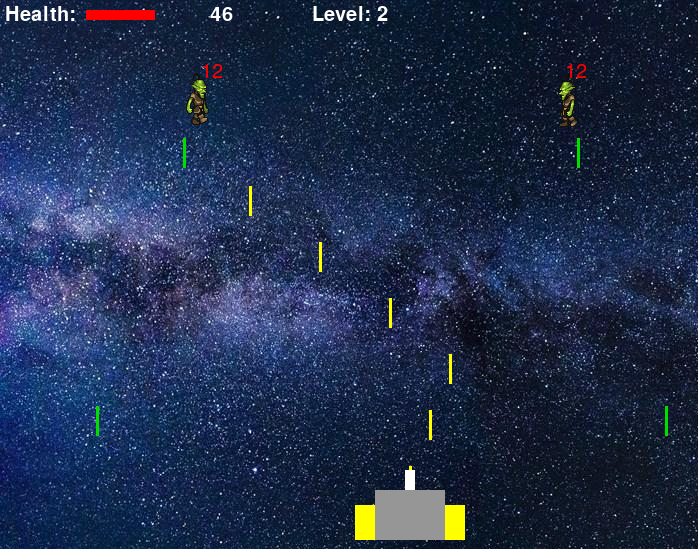
\includegraphics[scale=0.35]{screenshot.png}}
\caption{Screenshot of the Yellow-Spaceship game \cite{Yellow-Spaceship}.}
\label{fig:game_screenshot}
\end{figure}

The number of levels is not bound and the aim of the game is to kill as many enemies as
possible and reach the highest level without losing the whole life.
\section{Methodologies and Implementation}
Starting from the Yellow-Spaceship game \cite{Yellow-Spaceship}, we have adapted the code to our needs.
In particular, we have modified the code that reads the action from the user keyboard in order to be
able to substitute the user input with an action computed by a program and apply it to the game.
The controlling action can be computed by an ANN evolved using NEAT, or by a tree-based program evolved 
using GP, passing them the appropriate information about the current state of the game.
Moreover, the possibility to not show the game has been introduced in order to speed up the execution.

The inputs from the game environment for both NEAT and GP individuals are the following:
the $x$ coordinate of the battleship; the velocity of the battleship;
the $x$ coordinate of the first and second alien (if any, otherwise they are set to 0);
the $x$ and $y$ coordinates of the first and second closest lasers (if any, otherwise they are set to 0);
the $x$ coordinate of the enemy spaceship (if any, otherwise it is set to 0).
In this way, there are a total of 9 arguments of type float passed to the individuals as input that
can be used to decide the action to perform. 
The performance of an individual can be evaluated based on how much it moves on in the game.

The fitness function for the individuals of both the algorithms that we decided to use can be
formulated as follows:
\begin{equation}
\begin{split}
    fitness = & alien\_kills * 10 + \\
              & enemy\_spaceship\_kills * 50 + \\
              & \sum_{h \in battleships\_healths}^{} \frac{h}{50} + \\
              & \sum_{a \in aliens}^{} \frac{cur\_alien\_health - a.health}{cur\_alien\_health} * 10 + \\
              & \sum_{s \in enemy\_spaceships}^{} 50 - s.health
\end{split}
\end{equation}
where $alien\_kills$ is the number of aliens killed, 
$enemy\_spaceship\_kills$ is the number of enemy spaceships killed,
$battleship\_healths$ is a vector of battleship health at the beginning of each level and
$cur\_alien\_health$ is the initial alien health at the last level reached. 

The fitness function should be maximized and takes into account the number of aliens and
enemy spaceships killed, the battleship health at each level and the health of aliens and
enemy spaceships at the last level reached. There is no intermediate reward and the overall
fitness is returned at the end of simulation.

In order to handle cases in which the simulation takes too much time because the battleship
is not killed, we introduced a maximum threshold on the number of frames: the game will be
stopped after $1$ million frames. The threshold permits to prevent the execution from getting
stuck and also incentivizes the NEAT and GP algorithms to learn how to reach higher levels
with the same number of frames. When the best individual execution is shown,
this limit is released in order to obtain the actual fitness without interrupting the game.

To speed up the evolution process, individuals are evaluated only every 10 frames to obtain
the action to perform: the previous action is applied for the rest of 9 frames. This value
should be sufficient to permit the individual to have enough control over the battleship
actions and not be killed by enemies. In this way the evaluation process proceeds about 10
times faster and the battleship movements look smoother.


\subsection{NEAT}
The implementation is based on the NEAT-Python library \cite{NEAT-Python}, which is a pure Python
implementation of NEAT, with no dependencies other than the Python standard library.
We decided to evolve a feed forward neural network with the possibility of learning skip
connections instead of a recurrent neural network since the actual state of the game is
sufficient to evolve the neural network and no more information is required. The network has 6
output nodes and each of them encodes a particular action that the agent has to perform:
go left; go left and fire; stay still; stay still and fire; go right; go right and fire.
The output node with the maximum value is taken to decide the action to perform.

We decided to adopt the following algorithm parameters:
\begin{itemize}
    \item $num\_runs = 10$, $num\_generations = 200$ and $no\_fitness\_termination = True$
    \item $pop\_size = 100$ and $reset\_on\_extinction = True$
    \item $activation = sigmoid$ and $aggregation = sum$
    \item $conn\_add\_prob = 0.5$ and $conn\_delete\_prob = 0.5$
    \item $enabled\_default = True$ and $enabled\_mutate\_rate = 0.01$
    \item $feed\_forward = True$ and $initial\_connection = full\_nodirect$
    \item $node\_add\_prob = 0.2$ and $node\_delete\_prob = 0.2$
    \item $num\_inputs = 9$, $num\_hidden = 9$ and $num\_outputs = 6$
    \item $species\_fitness\_func = max$, $max\_stagnation = 20$ and $species\_elitism = 2$
    \item $elitism = 2$, $survival\_threshold = 0.2$ and $min\_species\_size = 2$
\end{itemize}

All the configuration parameters used by the algorithm can be modified in the configuration
file named 'configNEAT.txt' present in the root directory of the project.


\begin{figure*}[htbp]
\centerline{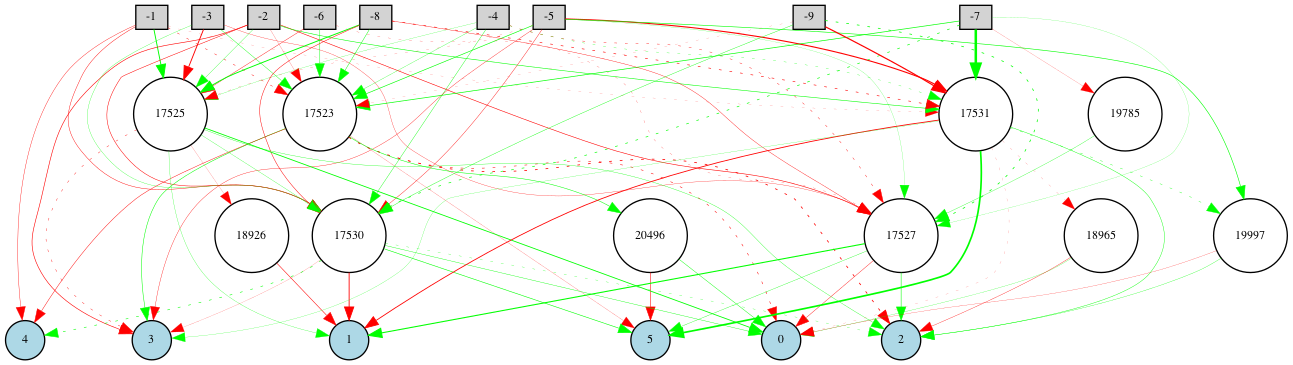
\includegraphics[scale=0.35]{NEAT_best.png}}
\caption{Best ANN generated by NEAT.}
\label{fig:NEAT_best}
\end{figure*}


\subsection{GP}
The implementation is based on the DEAP library \cite{DEAP}, which is a Python evolutionary
computation framework which provides the main blocks for building Genetic Programming
algorithms. Strongly typed genetic programming (STGP) is an enhanced version of genetic
programming which enforces data type constraints.

A tree-based program has been evolved using STGP. The output of the program is one of
the 6 encoded actions that the agent can perform. To encode the actions, we defined one
class for each of them with the following encoding:
A, go left; B, go left and fire; C, stay still; D, stay still and fire; E, go right; F, go right and fire.

The terminal set is composed of the action classes, some float values ($5$, $10$, $15$, $20$, $25$, $30$)
and the boolean values ("true", "false"). The function set is composed of the
boolean operators "greater than", "equal", "and", "or" and "negation", the arithmetic operators
"add", "subtract" and "multiply" and the "if\_then\_else" function that can outputs a float value or
an action class. Since the "if-then-else" function is the only function that outputs an action, it
should always be at the root of the tree.

We decided to adopt the following algorithm parameters:
\begin{itemize}
    \item $num\_runs = 10$ and $num\_generations = 200$
    \item $pop\_size = 100$
    \item $crossover\_prob = 0.5$
    \item $mutation\_prob = 0.5$
    \item $hof\_size = 4$
    \item $max\_tree\_size = 500$
    \item $max\_tree\_height = 10$
    \item As $expr\_init$ we used $gp.genFull$ with $min\_ = 1$ and $max\_ = 3$
    \item As $select$ we used $tools.selTournament$ with $tournsize = 7$
    \item As $mate$ we used $gp.cxOnePoint$
    \item As $expr\_mut$ we used $gp.genFull$ with $min\_ = 0$ and $max\_ = 2$
    \item As $mutate$ we used $gp.mutUniform$
    \item As $algorithm$ we used $deap.algorithms.eaSimple$
\end{itemize}

All the configuration parameters used by the algorithm can be modified in the configuration
file named 'configGP.txt' present in the root directory of the project.


\section{Results}
In this section we will present the results obtained with the two approaches and a
comparison between them and randomly piloted spaceships.

The evolution process stores at each run the best ANN or program generated with the
relative graphs in the folder 'runs' according to the specified approach. In this way it is
possible to relaunch them later and see through the graphical interface of the game how
they behave.

\subsection{NEAT}
The NEAT algorithm managed to evolve a ANN that can reach level 42 in the game with a
fitness of 1114 after about 160 generations. The ANN is represented in Fig. \ref{fig:NEAT_best}. As we can
see the network is quite simple, with a small number of nodes and connections: it has just 10
hidden nodes and 63 enabled connections.


\begin{figure}[h!]
\centerline{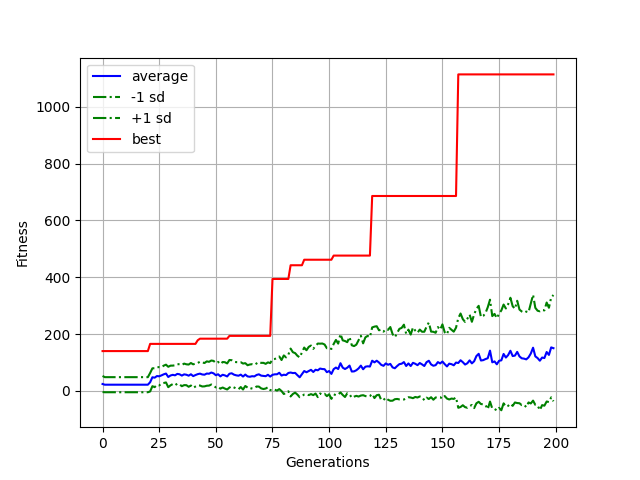
\includegraphics[scale=0.55]{NEAT_fitness.png}}
\caption{Fitness trend of the NEAT run that has generated the best ANN.}
\label{fig:NEAT_fitness}
\end{figure}


\begin{figure}[h!]
\centerline{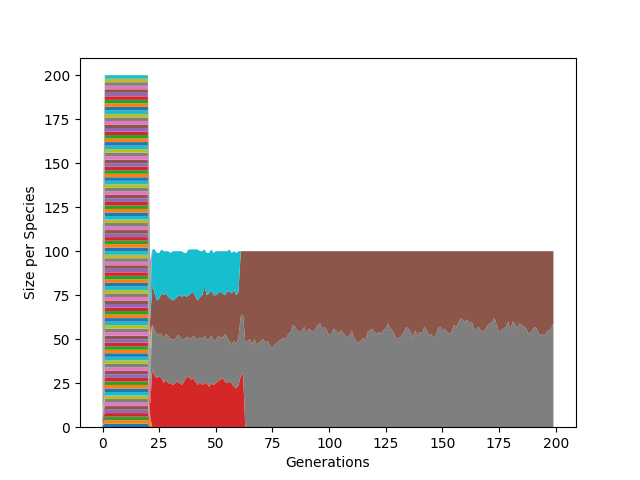
\includegraphics[scale=0.55]{NEAT_speciation.png}}
\caption{Speciation trend of the NEAT run that has generated the best ANN.}
\label{fig:NEAT_speciation}
\end{figure}

In Fig. \ref{fig:NEAT_fitness}, we can observe that the best fitness increases significantly in just a few particular
generations, whereas the average fitness does not grow significantly and stays under 200.
With this fitness trend, we can also notice that the speciation decreases significantly after 20
generations due to stagnation of a lot of species and just the 2 elitism species will survive
after about 60 generations as shown in Fig. \ref{fig:NEAT_speciation}.

A weak point of NEAT is that the generated ANN is not really interpretable and we cannot
understand why the network produces certain output values.


\subsection{GP}
The GP algorithm managed to evolve two tree-based programs that can reach over 4000 fitness in the simulation.
The first program reaches level 151 in the
game with a fitness of 4061 during the evolution process and level 194 and with a fitness of 5212
without limiting the number of frames. The tree of the program is represented in Fig. \ref{fig:GP_best1}. As
we can see the tree is quite complex, with 259 nodes and a depth of 10 (the maximum depth
allowed). In Fig. \ref{fig:GP_fitness1}, we can observe that the best fitness improves a lot in the first 60
generations reaching the frame threshold.
% ; in the remaining generations, the best fitness
% trend increases slightly, probably also due to this limitation to the number of frames. The
% average fitness trend is smoother and follows the best trend with a continuous increase: it
% reaches about 3000 fitness with a large variance (over 1000).
The second program reaches level 162 in the game with a fitness of 4342 during the evolution process and 
level 189 and with a fitness of 5076 without limiting the number of frames. The tree of the program is 
represented in Fig. \ref{fig:GP_best2}. As we can see the tree is a bit less complex than the first one, with 177 nodes 
and a depth of 10 (the maximum depth allowed). As shown in Fig. \ref{fig:GP_fitness2}, the best fitness improves significantly 
only after 100 generations, reaching the frame threshold.
In both cases, for the remaining generations, the best fitness trend increases slightly, probably also due 
to this limitation to the number of frames. The average fitness trend is smoother and follows the best trend 
with a similar increase, reaching about 3000 fitness with a large variance (over 1000).

A weak point of GP is that the generated tree is a bit complex and can be simplified a lot,
e.g. simplifying some 'if\_then\_else' statements with boolean values directly taken from the
terminal set ('true' or 'false') as conditions.

\begin{figure*}[t!]
    \centering
    \begin{subfigure}[b]{0.45\textwidth}
        \centering
        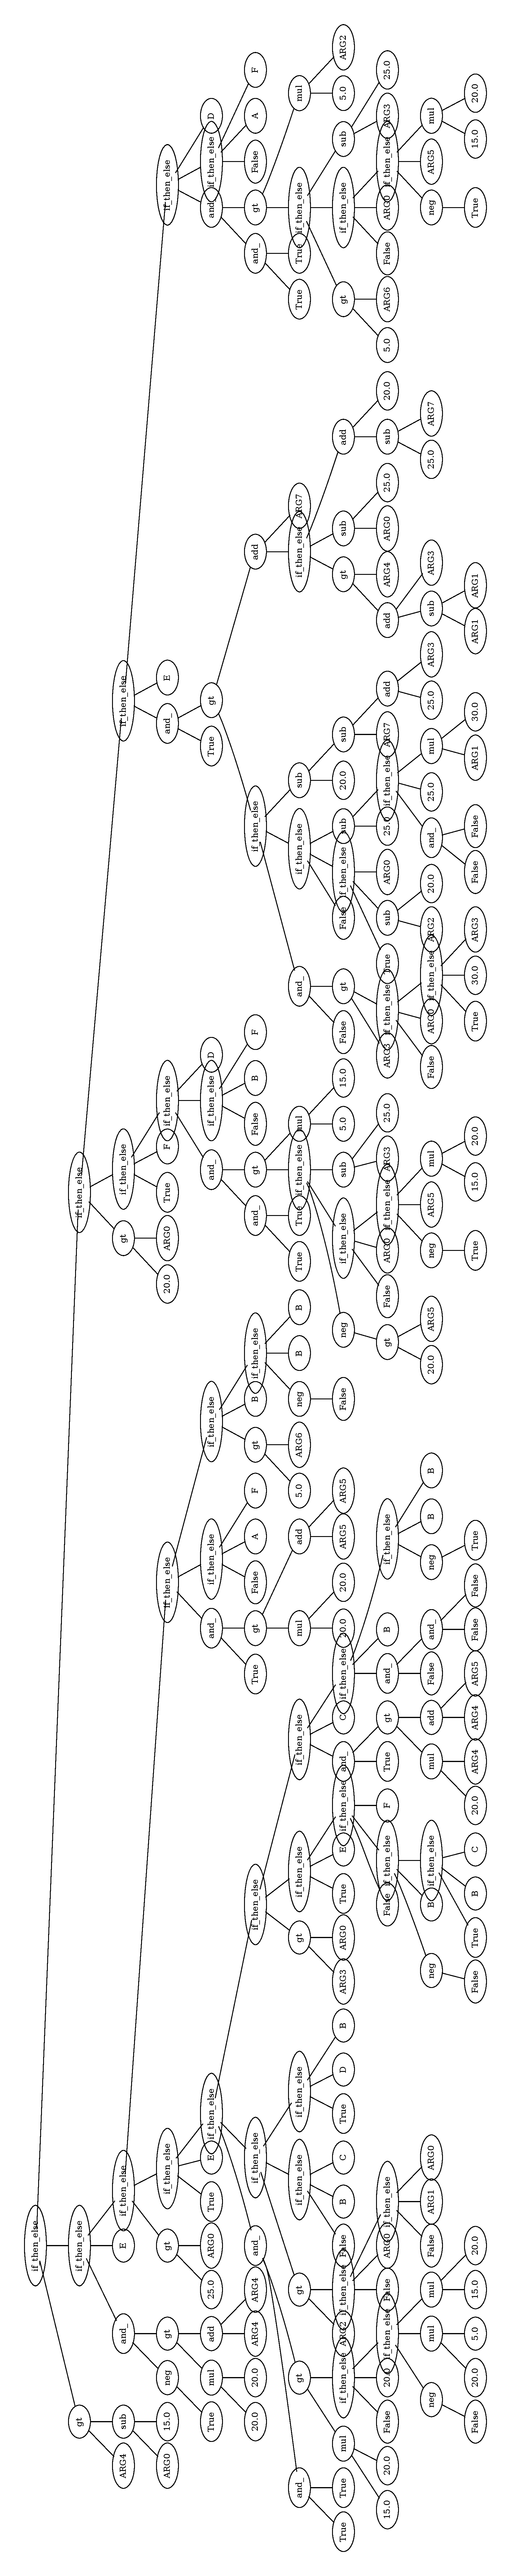
\includegraphics[scale=0.155]{GP_best1.pdf}
        \caption{}
        \label{fig:GP_best1}
    \end{subfigure}
    \hspace{1mm}
    \begin{subfigure}[b]{0.45\textwidth}
        \centering
        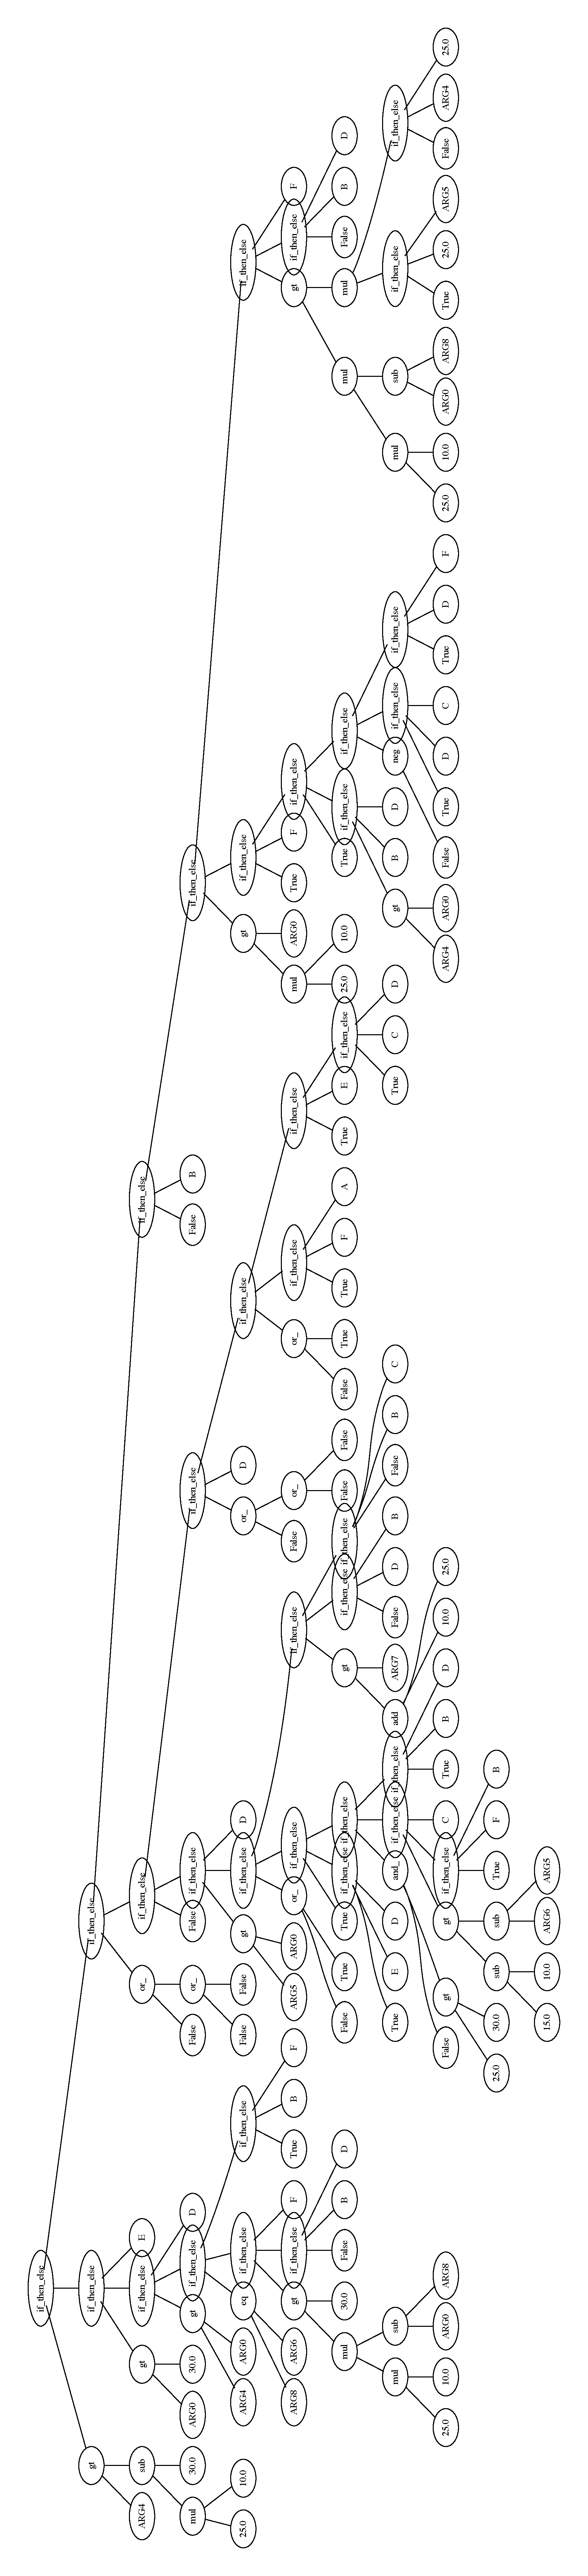
\includegraphics[scale=0.155]{GP_best2.pdf}
        \caption{}
        \label{fig:GP_best2}
    \end{subfigure}
       \caption{Best tree-based programs generated by GP.}
       \label{fig:GP_best}
\end{figure*}


\begin{figure*}[t!]
    \centering
    \begin{subfigure}[b]{0.45\textwidth}
        \centerline{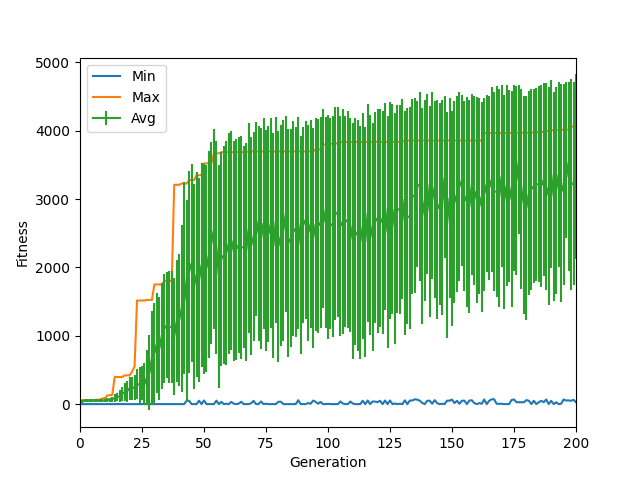
\includegraphics[scale=0.6]{GP_fitness1.png}}
        \caption{}
        \label{fig:GP_fitness1}
    \end{subfigure}
    \hfill
    \begin{subfigure}[b]{0.45\textwidth}
        \centerline{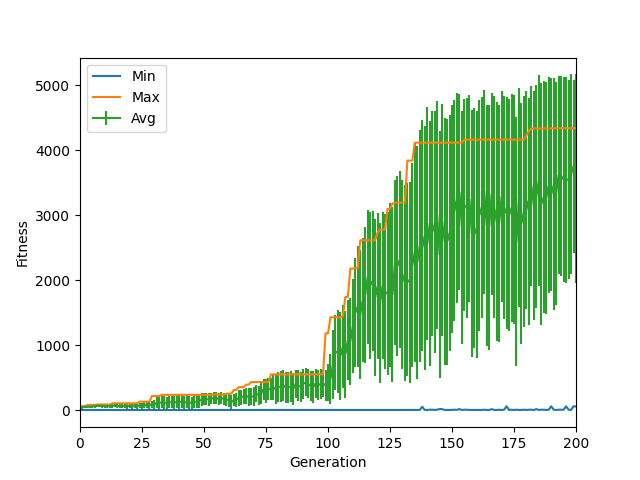
\includegraphics[scale=0.6]{GP_fitness2.png}}
        \caption{}
        \label{fig:GP_fitness2}
    \end{subfigure}
       \caption{Fitness trend of the GP runs that have generated the best programs.}
       \label{fig:GP_fitness}
\end{figure*}

% \begin{figure}[htbp]
% \centerline{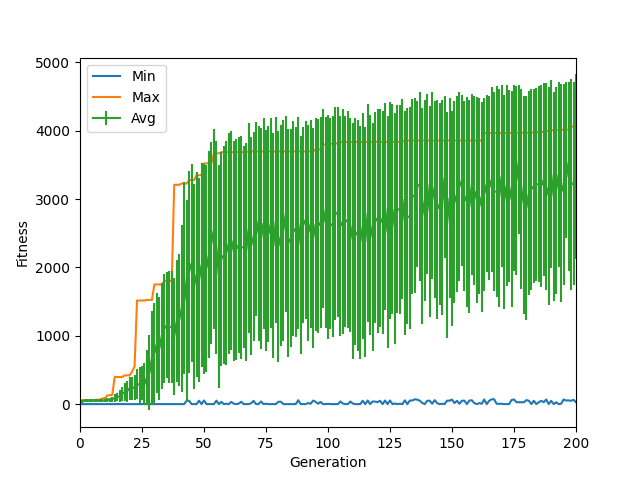
\includegraphics[scale=0.6]{GP_fitness1.png}}
% \caption{Fitness trend of the GP run that has generated the best program.}
% \label{fig:GP_fitness1}
% \end{figure}

% \begin{figure}[htbp]
% \centerline{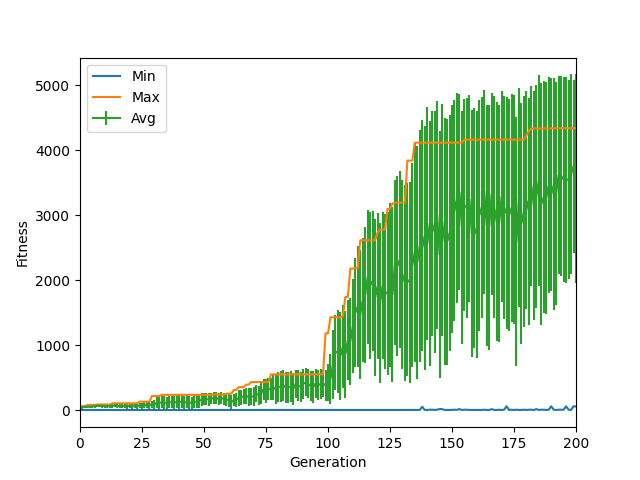
\includegraphics[scale=0.6]{GP_fitness2.png}}
% \caption{Fitness trend of the GP run that has generated the best program.}
% \label{fig:GP_fitness2}
% \end{figure}


\subsection{Comparison}
With both techniques, we managed to find a program that is able to play the game well,
learning to fire almost always to hit enemies while dodging their lasers.

GP demonstrated to have a bigger potential considering our scenario: thanks to the
tree-structure and the functions provided, it is able to learn more complex strategies
reaching level 194, much more than the best evolved ANN. NEAT, instead, struggles to
evolve the network reaching in the best only level 42. NEAT is probably more suitable for
different tasks when a program would not be the best option or even it would be impossible
to build.

Moreover, a tree with a limited size can be more interpretable than a ANN and we can easily
provide an explanation for what the agent is doing.

Observing the agent in action we can say that: both move quite smoother, even though
neither of them is human-like, GP looks smarter with respect to NEAT. In fact, GP has a
tendency to stay in the middle of the playing area dodging all the lasers, while NEAT tends to
remain in the corners.

Across multiple runs, NEAT seems to obtain more stable results than GP that only a few
times manages to reach very good results as shown in Fig. \ref{fig:boxplots}. Both the techniques are
pretty good and much better than a randomly piloted spaceship that on average is just able
to reach level 3.


% TODO: fix captions
\begin{figure*}
    \centering
    \begin{subfigure}[b]{0.3\textwidth}
        \centering
        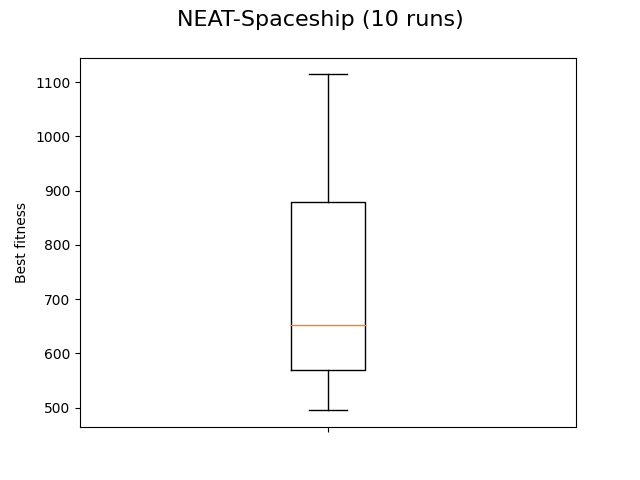
\includegraphics[scale=0.4]{NEAT_Boxplot.png}
        \caption{NEAT boxplot}
    \end{subfigure}
    \hspace{3mm}
    \begin{subfigure}[b]{0.3\textwidth}
        \centering
        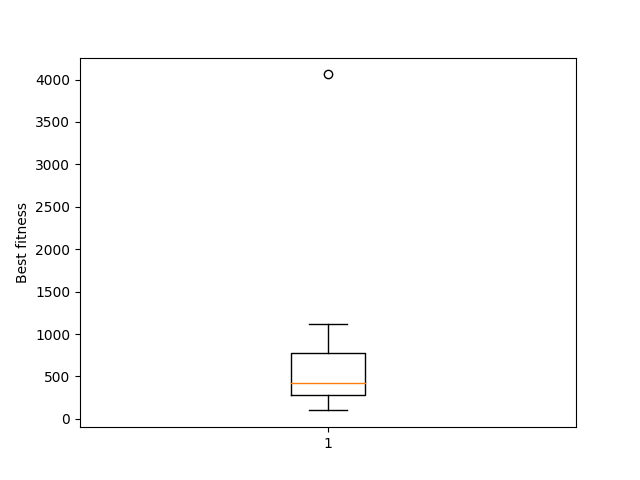
\includegraphics[scale=0.4]{GP_Boxplot.png}
        \caption{GP boxplot}
    \end{subfigure}
    \hspace{3mm}
    \begin{subfigure}[b]{0.3\textwidth}
        \centering
        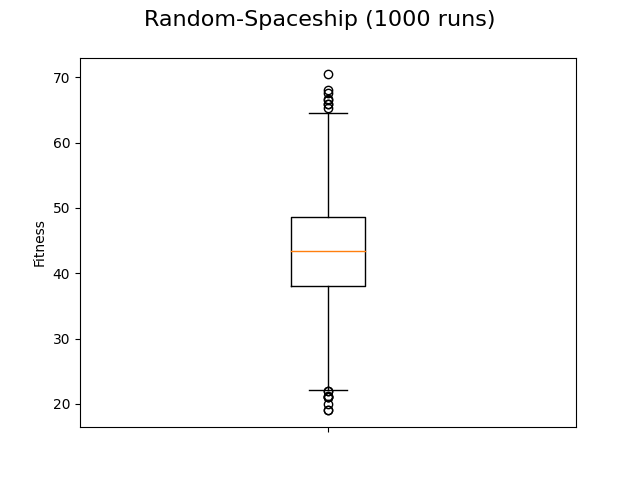
\includegraphics[scale=0.4]{Random_Boxplot.png}
        \caption{Random boxplot}
    \end{subfigure}
       \caption{Comparison between boxplots of NEAT, GP and randomly piloted spaceships.}
       \label{fig:boxplots}
\end{figure*}
\section{Conclusions}
Both are very good approaches and managed to find a way to play the game well. Even
though, across multiple runs, NEAT seems to obtain more stable results, GP has
demonstrated to have a bigger potential thanks to the tree-structured individuals and overall
manages to reach very good results.

One of the issues that we encountered using GP is how to manage the different input types:
one may implement functions taking into account inputs of different types or, alternatively,
one can use a strongly typed primitive set as we do.

Another issue we have is that the execution of the algorithms takes a lot of time and
computational resources, especially when the frame threshold is reached. Due to this, the
number of runs and individuals should be limited.

In the end, we learned a lot about this field from this project, in particular how it is possible to
apply bio-inspired techniques to real-world problems and how to benefit from it. They have
proved to be a valid alternative to classic back-propagation algorithms for ANN and in this
case we have finally learned new ways to do a kind of reinforcement learning using the
fitness as a reward.



% Can use something like this to put references on a page
% by themselves when using endfloat and the captionsoff option.
\ifCLASSOPTIONcaptionsoff
  \newpage
\fi

% references section

% can use a bibliography generated by BibTeX as a .bbl file
% BibTeX documentation can be easily obtained at:
% http://mirror.ctan.org/biblio/bibtex/contrib/doc/
% The IEEEtran BibTeX style support page is at:
% http://www.michaelshell.org/tex/ieeetran/bibtex/
%\bibliographystyle{IEEEtran}
% argument is your BibTeX string definitions and bibliography database(s)
%\bibliography{IEEEabrv,../bib/paper}
%
% <OR> manually copy in the resultant .bbl file
% set second argument of \begin to the number of references
% (used to reserve space for the reference number labels box)
\begin{thebibliography}{1}

\bibitem{Yellow-Spaceship}
https://github.com/ph3nix-cpu/Yellow-Spaceship

\bibitem{NEAT}
K. O. Stanley and R. Miikkulainen, "Evolving Neural Networks through Augmenting Topologies," in Evolutionary Computation, vol. 10, no. 2, pp. 99-127, June 2002, doi: 10.1162/106365602320169811.

\bibitem{GP}
Koza, John R. "Hierarchical genetic algorithms operating on populations of computer programs." IJCAI. Vol. 89. 1989.

\bibitem{NEAT-Python}
https://neat-python.readthedocs.io/en/latest/index.html

\bibitem{DEAP}
https://deap.readthedocs.io/en/master/index.html

\bibitem{PyGame}
https://www.pygame.org/docs/

\bibitem{repository}
https://github.com/samuelbortolin/Bio-Inspired-Spaceship

\end{thebibliography}

\end{document}


